\documentclass[12pt]{article}

\usepackage{amsmath}
\usepackage[hidelinks]{hyperref}
\usepackage{fancyhdr}
\usepackage{color}
\usepackage{titlesec}
\usepackage[pdftex]{graphicx}
\usepackage{datetime}

\pagestyle{fancy}
\fancyhf{}

% custom section
\titlespacing{\section}{0pt}{*2}{0pt}
\titleformat{\section}[runin]
{\normalfont\bfseries}
{\thesection. }
{0pt}
{}[\\]

\begin{document}

\fancyhead[L]
{
\textbf{Distributed Algorithms: Assignment 3 C}\\
Christos Froussios (4322754) \& Quinten Stokkink (4016270)\\
\today
}
\setlength\headheight{0.8in}
\setlength\topmargin{-0.6in}
\setlength\textheight{9.0in}
\setlength\parindent{0pt}

\section{Introduction}
In this report we present the results of our implemenation of Afek \& Gafni's algorithm for election in a completely connected network.
We use a slightly modified version of the algorithm to avoid drowning single processes in so many messages they slow down the
whole algorithm. This involves selecting from the untraversed link pool in a random order and a timeout between trying to capture
the same node successively. Furthermore we demote candidate processes that have been killed and have no outstanding messages
to just an ordinary process.

\section{Methodology}

\section{Results}

\begin{figure}[h]
    \centering
    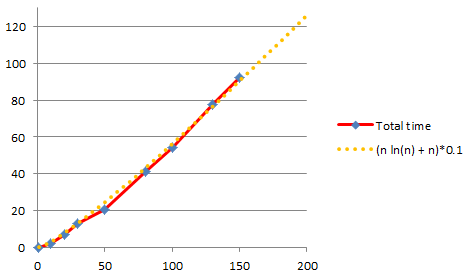
\includegraphics{totaltime.png}
    \caption{The total time taken for the algorithm to terminate versus the amount of processes}
    \label{fig:totaltime}
\end{figure}

\begin{figure}[h]
    \centering
    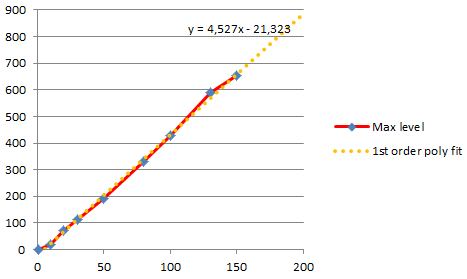
\includegraphics{maxlevel.png}
    \caption{The maximum level achieved versus the amount of processes}
    \label{fig:maxlevel}
\end{figure}

\end{document}